\chapter{1-Dimensional model}
\label{chapter:1-Dimensional}


\section{Setup}
We consider a system of two interacting quantum-mechanical electrons and a classical dipole. We take the electrons on the x-axis, a fixed distance $h$ apart from the dipole. Further, we assume a strong and constant electric field $E_0$ at an angle $\theta_0$ to the x-axis. The dipole has a dipole moment of $\mathbf{d}$, pointing in the direction of the total electric field, that being the sum of the external electric field and the electric field caused by the two electrons. It is further assumed all electric fields are screened, with a screening constant $\kappa$. This setup is shown in figure \ref{fig:setup}.

\begin{figure}[h]
    \centering
    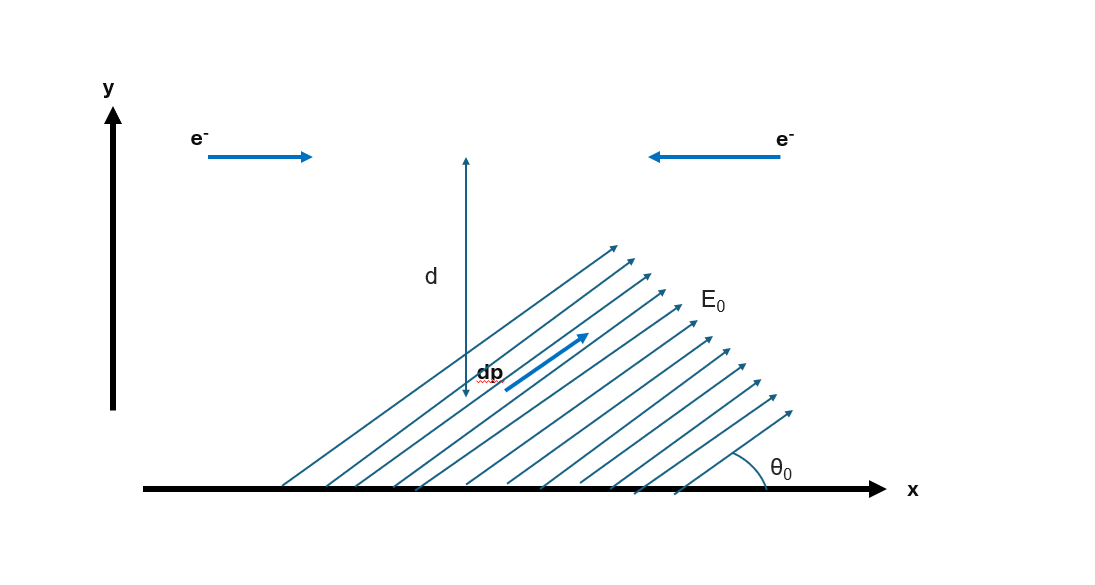
\includegraphics[width=0.5\textwidth]{figures/setup.png}
    \caption{Setup of the system. The dipole is at the origin, with the electrons at a distance $h$ from the dipole. The external electric field is at an angle $\theta_0$ to the x-axis.}
    \label{fig:setup}
\end{figure}

\section{Limiting cases}
To check the physical validity of a model, it is important to test for extreme values of parameters in a model, and see if they make intuitive and physical sense. 


\section{Attractive interaction}
The repulsive interaction between electrons due to Coulomb interaction is given by by the potential energy $V_\text{C}(x_1, x_2) = \frac{e^2}{4 \pi \epsilon_0 |x_1-x_2|}$ Taking the screening from ions into account we find $V_\text{C}(x_1, x_2) = \frac{e^2}{4 \pi \epsilon_0 |x_1-x_2|}e^{-\kappa|x_1-x_2|}$



The dipole is polarized by the presence of an external electric field. The electric field $\mathbf{E_0}$ is given by:
\begin{equation}
    \mathbf{E_0} = 
    E_0 (\cos(\theta_0) \hat{x} + \sin(\theta_0) \hat{y})
\end{equation}
Where $E_0$ is the magnitude of the electric field, and $\theta_0$ is the angle of the electric field to the x-axis. 

The electric field due to an electron at the location of the dipole is given by:
\begin{equation}
    \mathbf{E_{\text{e}_1}} = 
    \frac{e^-}{4 \pi \epsilon_0 (x_1^2+d^2)} \hat{r} 
\end{equation}
Where $\hat{r}$ is the unit vector pointing from the dipole to the electron, given by $\frac{x_1}{\sqrt{x_1^2+d^2}} \hat{x} + \frac{d}{\sqrt{x_1^2 + d^2}} \hat{y}$, and similar for $x_2$. This gives a total electric field at the dipole of 

\begin{align}
    \mathbf{E_{tot}} = 
    \begin{pmatrix}
        \cos(\theta_0) E_0 + \frac{e^-}{4 \pi \epsilon_0} 
        \left( \frac{x_1}{(x_1^2+d^2)^{3/2}} + \frac{x_2}{(x_2^2+d^2)^{3/2}} \right)  \\
        \sin(\theta_0) E_0 + \frac{e^-}{4 \pi \epsilon_0} 
        \left( \frac{d}{(x_1^2+d^2)^{3/2}} + \frac{d}{(x_2^2 + d^2) ^{3/2}} \right) 
    \end{pmatrix}
\end{align}

Since the dipole will try to align with the electric field, we find that the angle the dipole will make with the x-axis will be given by $\arctan{..., ...}$. By taking a taylor approximation of $\arctan(x)$, we find
\begin{equation}
    \arctan(x) = \sum_{n=0}^{\infty} \frac{(-1)^n}{2n+1}x^{2n+1}
\end{equation}
Which we approximate with $\arctan(x) \approx x$. 
Further, using $\cos(\theta_0) E_0 >> \frac{e^-}{4 \pi \epsilon_0}$, and using a Taylor approximation to find $\frac{d}{(x^2+d^2)^{3/2}} \approx \frac{1}{d^2} - \frac{3x^2}{2d^4}$. This leads to the following equation for $\theta$ 
\begin{equation}
    \theta = 
    \frac{\sin(\theta_0)E_0 + \frac{e^-}{4 \pi \epsilon_0}
    \left(\frac{2}{d^2}-\frac{3(x_1^2+x_2^2) }{2d^4}\right)}{\cos(\theta_0) E_0}
\end{equation}

We will expand $\arctan(x)$ around $x=\tan(\theta_0)$. Using $\frac{d}{dx} \arctan(x) = \frac{1}{1+x^2}$ and $\frac{d^2}{dx^2} \arctan(x) = \frac{-2x}{(1+x^2)^2}$, we find the second order approximation of $\arctan(x)$ around $x=\tan(\theta_0)$ to be $\arctan(x) \approx \theta_0 + \frac{x-\tan(\theta_0)}{1+\tan(\theta_0)^2} - \frac{\tan(\theta_0) (x-\tan(\theta_0))^2}{(1+\tan(\theta_0)^2)^2}$. From here, we disregard any terms higher than second order. This gets us

Using small angle approximations for $\sin(\theta)$ and $\cos(\theta)$

\section{Vector notation}
\label{section: Vector Notation}
Doing the same calculations using vector notation, we find the following. 
First, we have 
\begin{equation}
    \mathbf{E_0} = 
    \begin{pmatrix*}
        E_0 \cos(\theta_0) \\
        E_0 \sin(\theta_0)
    \end{pmatrix*}
\end{equation}
Assuming a screened electric field, we take the Yukawa potential 
\begin{equation}
    V_\kappa (\mathbf{r_i}) = \frac{(e^-)^2}{4 \pi \epsilon_0 r_i} e^{-\kappa r_i} 
\end{equation}
Where $\kappa$ is the screening constant, $r$ is the distance between the electron and the dipole, and $\mathbf{r}$ is the vector pointing from the dipole to the electron.
We want to know the electric field at the dipole. The electric field at the dipole due to an electron at position $\mathbf{r_i}$
\begin{equation}
    \mathbf{E} = - \nabla V_\kappa (\mathbf{r_i}) = 
    \frac{(e^-)^2}{4 \pi \epsilon_0} \frac{e^{-\kappa r_i}}{r_i} \left( \kappa + \frac{1}{r_i} \right) \hat{r_i}
\end{equation}

This would mean the dipole would point in the direction 
\begin{equation}
    \hat{d} = \hat{E} = 
    (\mathbf{E_0 + E_1 + E_2} ) / | \mathbf{E_0 + E_1 + E_2} |
\end{equation}
Where $\mathbf{E_0}$ is the externally applied electric field, $\mathbf{E_1}$ is the electric field due to the first electron, and $\mathbf{E_2}$ is the electric field due to the second electron. That gives a dipole moment of 
\begin{equation}
    \mathbf{d} = 
    d \hat{\mathbf{d}}
\end{equation}
Then the potential energy of the electrons due to the dipole is given by
\begin{equation}
    V_{\text{dp,i}} = 
    \frac{\mathbf{d} \cdot \mathbf{r_1}}{4 \pi \epsilon_0 |\mathbf{r_i}|^3}
\end{equation}
Including screening we find
\begin{equation}
    V_{\text{dp},i} = 
    \frac{\mathbf{d} \cdot \mathbf{r_i}}{4 \pi \epsilon_0 |\mathbf{r_i}|^3}
    e ^{-\kappa |\mathbf{r_i}|}
\end{equation}


Further, we have the interaction between the two electrons, given by 
\begin{equation}
    V_{\text{C}} = 
    \frac{e^-}{4 \pi \epsilon_0 |\mathbf{r_1} - \mathbf{r_2}|}
\end{equation}
Adding screening, we get
\begin{equation}
    V_{\text{C}} = 
    \frac{e^-}{4 \pi \epsilon_0 |\mathbf{r_1} - \mathbf{r_2}|} 
    e ^ {-\kappa |\mathbf{r_1} - \mathbf{r_2}|}
\end{equation}


\section{Hamiltonian}
When using the single dipole model, the Hamiltonian of the system consists of six parts and is give by:  This hamiltonian is given by $\hat{H} = \hat{H}_{\text{e}_1} + \hat{H}_{\text{e}_2} + \hat{H}_{\text{e}_1 , \text{e}_2} + \hat{H}_{\text{e}_1 , \text{dp}} + \hat{H}_{\text{e}_2 , \text{dp}} + \hat{H}_{\text{e}_1 , \text{F}} + \hat{H}_{\text{e}_2 , \text{F}}$

Where the terms are kinetic energy of electron 1, the kinetic energy of electron 2, the kinetic energy of the dipole, the interaction between the two electrons, the interaction between electron 1 and the dipole, and the interaction between electron 2 and the dipole respectively.

The kinetic energy for the electron in one dimension is given by $\hat{H}_{\text{e}_1} = -\frac{\hbar^2}{2m}\frac{\partial^2}{\partial x_1^2}$ and $\hat{H}_{\text{e}_2} = -\frac{\hbar^2}{2m}\frac{\partial^2}{\partial x_2^2}$

Where $x_1$ and $x_2$ are the position of electron 1 and electron 2 respectively.
The kinetic energy for the dipole is given by $\hat{H}_{\text{dp}} = -\frac{\hbar^2}{2I}\frac{\partial^2}{\partial \theta^2}$

The interaction between the two electrons is given by $\hat{H}_{\text{e}_1 , \text{e}_2} = V_\text{C}(x_1, x_2)$

The interaction between electron 1 and the dipole is given by $\hat{H}_{\text{e}_1 , \text{dp}} = \frac{pq  e^-}{4 \pi \epsilon_0 (x_1^2 + d^2)^{3/2}} (x_1 \cos(\theta) + d \sin(\theta))$

The interaction between electron 2 and the dipole is given by $\hat{H}_{\text{e}_2 , \text{dp}} = \frac{p \cos(\theta)}{4 \pi \epsilon_0 x_2^2}$

The interaction between electron 1 and the external electric field is given by $\hat{H}_{\text{e}_1 , \text{F}} = -e E_0 \cos(\theta)$

The interaction between electron 2 and the external electric field is given by $\hat{H}_{\text{e}_2 , \text{F}} = -e E_0 \cos(\theta)$

These two terms will given a constant offset energy, and are therefore not relevant.

Finally, the interaction between the dipole and the external electric field is given by $\hat{H}_{\text{dp} , \text{F}} = -p E_0 \cos(\theta - \theta_0)$, where $\theta_0$ is the angle the external electric field makes with the x-axis.

Now the goal is to find a state with an energy $\langle{\psi(x_1, x_2, \theta)|\hat{H}|\psi(x_1, x_2, \theta)}\rangle < E_F$

The fermi energy is the energy of the

So first of all, one electron needs to be closer to the dipole than the other, to cause a rotation in the dipole. So we know the dipole is in a state rotated towards, say, positive x. Then electron 1, to the left of the dipole, is it a reasonably large distance from the dipole. Electron 2, to the right of the dipole, is at a reasonably small distance from the dipole. So let's say they're all Gaussian, with $\theta$ centered at $\pi / 4$, $x_1$ at a distance of -1, and $x_2$ at a distance of 0.5.

Let's fill this into the Hamiltonian, and not worry about complex coefficients or normalization for now?

\section{Hamiltonian vector notation}
Now that we have the interaction between electrons mediated by the dipole, we can give the Hamiltonian of the system. This Hamiltonian consists of five parts: The kinetic energies of each electron, the interaction of the electrons through the Coulomb force, the interaction mediated by the dipole, and the interaction with the external electric field. This leads to a Hamiltonian $\hat{H} = \hat{H}_{\text{e}_1} + \hat{H}_{\text{e}_2} + \hat{H}_{\text{C}} + \hat{H}_{\text{dp}} + \hat{H}_\text{E}$
Where the terms are the kinetic energy of each electron, the Coulomb interaction, the dipole mediated interaction, and the external electric field interaction respectively.  

\section{Normal solution}
Now let's try find a state with negative energy. Due to the coulomb interaction between electrons, unentangled electrons do not give a convergent solution. Therefore, we try the entangled state $\psi(x_1, x_2) = e^\frac{-(x_1-a_1)^2-(x_2-a_2)^2}{b}(x_1-x_2)$ with normalization constant $\frac{\pi}{4}b(2(a_1-a_2)^2 + b)$. $|\psi(x_1, x_2)|^2$ is shown in figure \ref{fig:phi_squared}
\begin{figure}[h]
    \centering
    \includesvg[width = \linewidth]{figures/phi_squared.svg}
    \caption{Schematic representation of electron-electron interaction mediated by a phonon with momentum \textbf{q} = \textbf{k-k'}}
    \label{fig:phi_squared}
\end{figure} 

To calculate the kinetic energy terms, we want to take the Fourier transform of the wavefunction. To transform $\psi(x_1, x_2)$ into a function of momenta, $\phi(p_1, p_2)$, we use
\begin{equation}
    \mathcal{F}\{\psi(x_1, x_2)\}(p_1, p_2) = 
    \int_{-\infty}^{\infty} 
    \int_{-\infty}^{\infty} \psi(x_1, x_2)e^{\frac{-i}{\hbar} (p_1 x_1 + p_2 x_2)}dx_1 dx_2 
\end{equation} 
Where $p_i = \hbar k_i$ is the quantum mechanical momentum.
This gives us
\begin{equation}
    \begin{split}
        \phi(p_1, p_2) = 
        \int_{-\infty}^{\infty} x_1 e^{-\frac{1}{b}x_1^2 + (\frac{2 a_1}{b} - \frac{i p_1}{\hbar}) x_1 - \frac{a_1^2}{b}} dx_1 
        \int_{-\infty}^{\infty} e^{-\frac{1}{b}x_2^2 + (\frac{2 a_2}{b} - \frac{i p_2}{\hbar}) x_2 - \frac{a_2^2}{b}} dx_2 \\ - 
        \int_{-\infty}^{\infty} x_2 e^{-\frac{1}{b}x_2^2 + (\frac{2 a_2}{b} - \frac{i p_2}{\hbar}) x_2 - \frac{a_2^2}{b}} dx_2 
        \int_{-\infty}^{\infty} e^{-\frac{1}{b}x_1^2 + (\frac{2 a_1}{b} - \frac{i p_1}{\hbar}) x_1 - \frac{a_1^2}{b}} dx_1 
    \end{split}
\end{equation}

Which evaluates to 
\begin{equation}
    \phi(p_1, p_2) = 
    (\frac{-a_1}{b}+\frac{ip_1}{2 \hbar} + \frac{a_2}{b} - \frac{i p_2}{2 \hbar}) \pi b^2 
    e^{- \frac{a_1^2}{b} + (\frac{a_1}{2 \sqrt{b}} - \frac{i \sqrt{b} p_1}{2 \hbar})^2} 
    e^{- \frac{a_2^2}{b} + (\frac{a_2}{2 \sqrt{b}} - \frac{i \sqrt{b} p_2}{2 \hbar})^2}
\end{equation}

Now, to use this to calculate the potential energy, we need to take it times its conjugate.
We find
\begin{equation}
    |\phi(p_1, p_2)|^2 = 
    \pi^2 b^4 \left(\frac{(a_2-a_1)^2}{b} + \frac{(p_1 - p_2)^2}{4 \hbar^2} \right) 
    e^{-\frac{a_1^2}{2b} -\frac{bp_1^2}{2\hbar^2}}
    e^{-\frac{a_2^2}{2b} - \frac{bp_2^2}{2\hbar^2}}
\end{equation}

\section{Relative Coordinates}
It can be useful to describe systems using different coordinates. To this end, we introduce the relative coordinate system. Here, we define $r = r_2 - r_1$ and $R = \frac{r_1 + r_2}{2}$. With this transformation, we also get new momentum coordinates. Defining $q = -i \hbar \frac{\partial}{\partial r}$ and $p = - i \hbar \frac{\partial}{\partial R}$, we find $q = \frac{p_1 - p_2}{2}$ and $p = p_1 + p_2$, where $p_1 = -i \hbar \frac{\partial}{\partial r_1}$ and $p_2 = -i \hbar \frac{\partial}{\partial r_2}$. 

This gives us interaction terms as follows:

With the wavefunction
$\phi(r, R) = e^{
    \frac{-2}{b}(R-\frac{1}{2}(a_1+a_2))^2+
    \frac{-1}{2b}(r+(a_1-a_2))^2+
    \frac{-1}{b}(a_1+a_2)^2}r$
Which becomes seperable into $f(r)g(R) = 
e^{\frac{-1}{2b}(r+(a_1-a_2))^2}r
e^{\frac{-2}{b}(R-\frac{1}{2}(a_1+a_2))^2}$
With normalization constant $\frac{1}{2}(2 (a_2-a_1)^2 + b) \sqrt{\pi b}$ for $f(r)$ and normalization constant $\frac{\sqrt{b \pi}}{2}$ for $g(R)$
Relative coordinates also change the interaction terms:
$V_C = \frac{e^-}{4\pi \epsilon_0 r} e ^{-\kappa r}$
We get $\hat{d} = \mathbf{E_0} + \mathbf{E_1} + \mathbf{E_2}$
Which results in a wavefunction looking like figure \ref{fig:relative_wf}

\begin{figure}[h]
    \centering
    \includesvg[width = \linewidth]{figures/relative_wf}
    \caption{Trial wavefunction $\psi$ in relative coordinates}
    \label{fig:relative_wf}
\end{figure}